% !TEX spellcheck = en_US
% !TEX spellcheck = LaTeX
\documentclass[letterpaper,english,10pt]{article}
\usepackage{%
	amsfonts,%
	amsmath,%	
	amssymb,%
	amsthm,%
	babel,%
	bbm,%
	%biblatex,%
	caption,%
	centernot,%
	color,%
	enumerate,%
	%enumitem,%
	epsfig,%
	epstopdf,%
	etex,%
	fancybox,%
	framed,%
	fullpage,%
	%geometry,%
	graphicx,%
	hyperref,%
	latexsym,%
	mathptmx,%
	mathtools,%
	multicol,%
	pgf,%
	pgfplots,%
	pgfplotstable,%
	pgfpages,%
	proof,%
	psfrag,%
	%subfigure,%	
	tikz,%
	times,%
	ulem,%
	url,%
	xcolor,%
	mathpazo
}

\definecolor{shadecolor}{gray}{.95}%{rgb}{1,0,0}
\usepackage[margin=1in,top=0.75in]{geometry}
\usepackage[mathscr]{eucal}
\usepgflibrary{shapes}
\usepgfplotslibrary{fillbetween}
\usetikzlibrary{%
  arrows,%
  backgrounds,%
  chains,%
  decorations.pathmorphing,% /pgf/decoration/random steps | erste Graphik
  decorations.text,% 
  matrix,%
  positioning,% wg. " of "
  fit,%
  patterns,%
  petri,%
  plotmarks,%
  scopes,%
  shadows,%
  shapes.misc,% wg. rounded rectangle
  shapes.arrows,%
  shapes.callouts,%
  shapes%
}

%\pgfplotsset{compat=newest} %<------ Here
\pgfplotsset{compat=1.11} %<------ Or use this one

\theoremstyle{plain}
\newtheorem{thm}{Theorem}[section]
\newtheorem{lem}[thm]{Lemma}
\newtheorem{prop}[thm]{Proposition}
\newtheorem{cor}[thm]{Corollary}
\newtheorem{clm}[thm]{Claim}

\theoremstyle{definition}
\newtheorem{axiom}[thm]{Axiom}
\newtheorem{defn}[thm]{Definition}
\newtheorem{conj}[thm]{Conjecture}
\newtheorem{exmp}[thm]{Example}
\newtheorem{exerc}[thm]{Exercise}
\newtheorem{assum}[thm]{Assumptions}

\theoremstyle{remark}
\newtheorem{rem}[thm]{Remark}
\newtheorem{note}[thm]{Note}

\newcommand{\Cov}{\operatorname{Cov}}
%\newcommand{\det}{\operatorname{det}}
\newcommand{\Real}{\mathbb{R}}
\newcommand{\tr}{\operatorname{tr}}
%\newcommand{\Var}{\operatorname{Var}}

\DeclareMathOperator{\sign}{sign}
%\renewcommand{\proof}[1]{\begin{proof}#1\end{proof}}
\newcommand{\EQ}[1]{\begin{equation*}#1\end{equation*}}
\newcommand{\EQN}[1]{\begin{equation}#1\end{equation}}
\newcommand{\eq}[1]{\begin{align*}#1\end{align*}}
\newcommand{\meq}[2]{\begin{xalignat*}{#1}#2\end{xalignat*}}
\newcommand{\norm}[1]{\left\lVert#1\right\rVert}
\newcommand{\abs}[1]{\left\lvert#1\right\rvert}
\newcommand{\expect}[1]{\mathbb{E}\left[{#1}\right]}
\newcommand{\prob}[1]{\mathbb{P}\left[{#1}\right]}
\newcommand{\given}{\; \big\vert \;} 
\newcommand{\set}[1]{\left\{#1\right\}} 
\newcommand{\indicator}[1]{\mathbb{1}_{\set{#1}}} 
\newcommand{\inner}[1]{\left\langle#1\right\rangle}
\newcommand{\red}[1]{\textcolor{red}{#1}} 
\newcommand{\E}[1]{\mathbb{E}\left[#1\right]}
\newcommand{\Var}[1]{\operatorname{Var}\left[#1\right]}

\newcommand{\D}{\mathbb{D}}
%\newcommand{\E}{\mathbb{E}}
\newcommand{\N}{\mathbb{N}}
\renewcommand{\P}{\mathbb{P}}
\newcommand{\Q}{\mathbb{Q}}
\newcommand{\R}{\mathbb{R}}
\newcommand{\Z}{\mathbb{Z}}

\newcommand{\bU}{\mathbf{1}}
\newcommand{\bx}{\mathbf{x}}

\newcommand{\cB}{\mathcal{B}}
\newcommand{\cC}{\mathcal{C}}
\newcommand{\cD}{\mathcal{D}}
\newcommand{\cF}{\mathcal{F}}
\newcommand{\cG}{\mathcal{G}}
\newcommand{\cH}{\mathcal{H}}
\newcommand{\cO}{\mathcal{O}}
\newcommand{\cT}{\mathcal{T}}
\newcommand{\cX}{\mathcal{X}}
\newcommand{\cY}{\mathcal{Y}}

\newcommand{\sA}{\mathscr{A}}
\newcommand{\sB}{\mathscr{B}}
\newcommand{\sC}{\mathscr{C}}
\newcommand{\sD}{\mathscr{D}}
\newcommand{\sE}{\mathscr{E}}
\newcommand{\sF}{\mathscr{F}}
\newcommand{\sG}{\mathscr{G}}
\newcommand{\sH}{\mathscr{H}}
\newcommand{\sL}{\mathscr{L}}
\newcommand{\dO}{\mathscr{O}}
\newcommand{\sS}{\mathscr{S}}
\newcommand{\sT}{\mathscr{T}}
\newcommand{\sX}{\mathscr{X}}
\newcommand{\sY}{\mathscr{Y}}
\newcommand{\sZ}{\mathscr{Z}}

% Debug
\newcommand{\todo}[1]{\begin{color}{blue}{{\bf~[TODO:~#1]}}\end{color}}

% a few handy macros

\renewcommand{\le}{\leqslant}
\renewcommand{\ge}{\geqslant}
\newcommand\matlab{{\sc matlab}}
\newcommand{\goto}{\rightarrow}
\newcommand{\bigo}{{\mathcal O}}
%\newcommand{\half}{\frac{1}{2}}
%\newcommand\implies{\quad\Longrightarrow\quad}
\newcommand\reals{{{\rm l} \kern -.15em {\rm R} }}
\newcommand\complex{{\raisebox{.043ex}{\rule{0.07em}{1.56ex}} \hskip -.35em {\rm C}}}


% macros for matrices/vectors:

% matrix environment for vectors or matrices where elements are centered
\newenvironment{mat}{\left[\begin{array}{ccccccccccccccc}}{\end{array}\right]}
\newcommand\bcm{\begin{mat}}
\newcommand\ecm{\end{mat}}

% matrix environment for vectors or matrices where elements are right justifvied
\newenvironment{rmat}{\left[\begin{array}{rrrrrrrrrrrrr}}{\end{array}\right]}
\newcommand\brm{\begin{rmat}}
\newcommand\erm{\end{rmat}}

% for left brace and a set of choices
%\newenvironment{choices}{\left\{ \begin{array}{ll}}{\end{array}\right.}
\newcommand\when{&\text{if~}}
\newcommand\otherwise{&\text{otherwise}}
% sample usage:
%  \delta_{ij} = \begin{choices} 1 \when i=j, \\ 0 \otherwise \end{choices}


% for labeling and referencing equations:
\newcommand{\eql}{\begin{equation}\label}
\newcommand{\eqn}[1]{(\ref{#1})}
% can then do
%  \eql{eqnlabel}
%  ...
%  \end{equation}
% and refer to it as equation \eqn{eqnlabel}.  


% some useful macros for finite difference methods:
\newcommand\unp{U^{n+1}}
\newcommand\unm{U^{n-1}}

% for chemical reactions:
\newcommand{\react}[1]{\stackrel{K_{#1}}{\rightarrow}}
\newcommand{\reactb}[2]{\stackrel{K_{#1}}{~\stackrel{\rightleftharpoons}
   {\scriptstyle K_{#2}}}~}


\makeatletter
\def\th@plain{%
  \thm@notefont{}% same as heading font
  \itshape % body font
}
\def\th@definition{%
  \thm@notefont{}% same as heading font
  \normalfont % body font
}
\makeatother
\date{}

%opening
\title{Lecture-08: Ferromagnets and Ising Model}

\begin{document}
\maketitle
\section{Ferromagnets and Ising models}
Magnetic materials contain molecules with individual magnetic moments, that tend to align the external magnetic field felt by the molecule. 
Magnetic moments of different molecules interact with each other. 
In many materials, the energy is lower when the moments align. 

A simple mathematical model for considering a number of particles with interacting moments is the Ising model, which describes the magnetic moments by Ising spins localized at the vertices of a certain region of a $d$-dimensional cubic lattice $\L$. 
The cubic lattice $\L$ is determined by the vertices $[L]^d$ and the edges $((i,j) \in [L]^d \times [L]^d: \sum_{k=1}^d\abs{i_k-j_k} = 1)$ between the nearest neighbors.  
At each coordinate $i \in [L]^d$, the configuration of a particle is an Ising spin $\sigma_i \in \sX = \{-1,1\}$. 
We have shown an example configuration of Ising spins for $L=5$ and $d=2$ in Figure~\ref{figure:IsingSpins}. 

%\red{Insert figure here}
\begin{figure}
\centering
\begin{tikzpicture}
\tikzstyle{spin}=[line width=0.4mm,draw=red,-triangle 45, postaction={draw, line width=1mm, shorten >=1.5mm, -}]

\draw [thick, draw=black, fill=white] (0,0) grid  (4,4) rectangle (0,0);

\draw [spin](0,4.3)--(0,3.7);
\draw [spin](1,4.3)--(1,3.7);
\draw [spin](2,4.3)--(2,3.7);
\draw [spin](3,3.7)--(3,4.3);
\draw [spin](4,3.7)--(4,4.3);

\draw [spin](0,3.3)--(0,2.7);
\draw [spin](1,3.3)--(1,2.7);
\draw [spin](2,2.7)--(2,3.3);
\draw [spin](3,3.3)--(3,2.7);
\draw [spin](4,3.3)--(4,2.7);

\draw [spin](0,1.7)--(0,2.3);
\draw [spin](1,1.7)--(1,2.3);
\draw [spin](2,1.7)--(2,2.3);
\draw [spin](3,2.3)--(3,1.7);
\draw [spin](4,2.3)--(4,1.7);

\draw [spin](0,1.3)--(0,0.7);
\draw [spin](1,1.3)--(1,0.7);
\draw [spin](2,0.7)--(2,1.3);
\draw [spin](3,0.7)--(3,1.3);
\draw [spin](4,1.3)--(4,0.7);

\draw [spin](0,0.3)--(0,-0.3);
\draw [spin](1,0.3)--(1,-0.3);
\draw [spin](2,0.3)--(2,-0.3);
\draw [spin](3,0.3)--(3,-0.3);
\draw [spin](4,0.3)--(4,-0.3);
\end{tikzpicture}

\caption{A configuration of a two-dimensional Ising model with L = 5. There is an Ising spin $\sigma_i$ on each vertex $i$, shown by an arrow pointing up if $\sigma_i = 1$ and pointing down if $\sigma_i = -1$.
The energy~\eqref{eqn:EnergyOfNparticleConfig}  is given by the sum of two types of contributions: 
$(i)$ a term $-\sigma_i\sigma_i$ for each edge $(i, j)$ of the graph, such that the energy is minimized when the two neighboring spins $\sigma_i$ and $\sigma_j$ point in the same direction; 
and $(ii)$ a term $-B\sigma_i$ for each site $i$, due to the coupling to an external magnetic field. 
The configuration shown here has an energy $-8+9B$.}
\label{figure:IsingSpins}
\end{figure}

\subsection{Energy function}
Let $N = L^d$, then the $N$ particle system configuration $\sigma$ is given by assigning the values of spins  for each of the $N$ particles as $\sigma = (\sigma_1, \sigma_2, \dots, \sigma_N)$. 
The space of configuration is $\sX^N = \{-1,1\}^N$. 
The energy of an $N$ particle configuration $\sigma$ is given by
\EQN{
\label{eqn:EnergyOfNparticleConfig}
E(\sigma) = - \sum_{(i,j)} \sigma_i \sigma_j - B \sum_{i \in [L]^d} \sigma_i.
}
where the sum over $(i,j)$ runs over all the unordered pairs of sites $i,j \in [L]^d$ which are nearest neighbors and $B$ is the applied external magnetic field. 


Determining the free energy density $f(\beta)$ in the thermodynamic limit for this model is a non-trivial task. In 1924, Ernst Ising solved the $d=1$ case and showed the absence of phase transitions. 
In 1948, Lars Onsager solved the $d=2$ case, exhibiting the first soluble `finite-dimensional' model with a second-order phase transition. 
In higher dimensions, the problem is unsolved, although many important features of the solution are well understood.

\subsection{Temperature limits}
The two limiting cases that can be considered are at high and low temperatures. 
At high temperature when $\beta \to 0$, the energy no longer matters and the Boltzmann distribution is uniform over all configurations $\sigma \in \sX^N$. 
That is, 
\EQ{
\mu_\beta (\sigma) = \frac{1}{2^N}. 
}
At low temperature when $\beta \to \infty$, 
the Boltzmann distribution concentrates onto the ground state(s). 
In the absence of external magnetic field, i.e $B=0$, the two degenerate ground states are given by,
\meq{2}{
&\sigma_+ = (\sigma_i = 1: i \in [L]^d),&
&\sigma_- = (\sigma_i = -1: i \in [L]^d).
}
If the magnetic field is set to some non-zero value, one of the two configuration dominates. 
The ground state is $\sigma_+$ if $B>0$ and the ground state is $\sigma_-$ if $B<0$.
%
%\subsection{}
%In an earlier discussion on Ising model, some of its qualitative properties were studied. The energy in the two limiting cases - infinite temperature ($\beta \to 0$) and zero temperature ($\beta \to \infty$) - were briefly discussed. It was learnt that temperature impacts the energy of the system, and thereby the spins. In the high-temperature limit there were no spin patterns, and the configurations were uniformly random. However, in the low-temperature limit the response of the system - configurations with all spins pointing up and/or down - was determined by the presence or absence of an external magnetic field ($B$). 
To analyse this behavior upon the application of a magnetic field, 
We define a \textit{rescaled} magnetic field $x=\beta B$, with $\beta \to 0$ or $\beta \to \infty$, keeping $x$ fixed. 
With this, we will subsequently study some of the qualitative properties of the resultant model.

\begin{defn}[Expected Spin] Consider a ferromagnetic Ising model whose energy function is given by,
$$E(\underline{\sigma}) = -\sum_{(ij)}\sigma_{i}\sigma_{j} - B \sum_{i\in \mathbb{L}}\sigma_{i}.$$
Let us assume that the spins are non-interacting, then, the total energy of the system due to all possible configurations is given by,
\begin{equation}
E(\underline{\sigma}) = - B \sum_{i\in \mathbb{L}}\sigma_{i}.
\end{equation}
The corresponding partition function is
\begin{align}
Z(\beta) &= \sum_{\underline{\sigma}}\exp(-\beta E(\underline{\sigma})),\nonumber\\  
Z(\beta) &= \sum_{\sigma_{1}=\sigma_{2}=\ldots=\sigma_{N} = \pm 1}\exp(\beta B \sum_{i\in \mathbb{L}}\sigma_{i}).
\end{align}
The partition function for a single spin with energy            $E(\sigma_{i}) = -B\sigma_{i}$ is therefore,
\begin{align}
Z_{i}(\beta) &= \sum_{\sigma_{i} = \pm 1}\exp(-\beta E(\sigma_{i})),\nonumber\\  
Z_{i}(\beta) &= e^{\beta B}+ e^{-\beta B},\nonumber\\
Z_{i}(\beta) &= 2\cosh(\beta B).
\end{align}
At each site, the probability of an up spin or a down spin is given by Boltzmann's distribution,
\begin{align}
P(\sigma_{i}) &= \frac{\exp(-\beta E(\sigma_{i}))}{Z_{i}(\beta)}.
\end{align}
Therefore, the average value of a single spin in a region $\mathbb{L}$ is
\begin{align}
\langle\sigma_{i}\rangle &= \sum_{\sigma_{i}=\pm 1}P(\sigma_{i})\sigma_{i},\nonumber\\
\langle\sigma_{i}\rangle &= \frac{e^{\beta B}-e^{-\beta B}}{Z_{i}(\beta)},\nonumber\\
 \langle\sigma_{i}\rangle &= \tanh(\beta B).
\end{align}
\begin{figure}
\centering
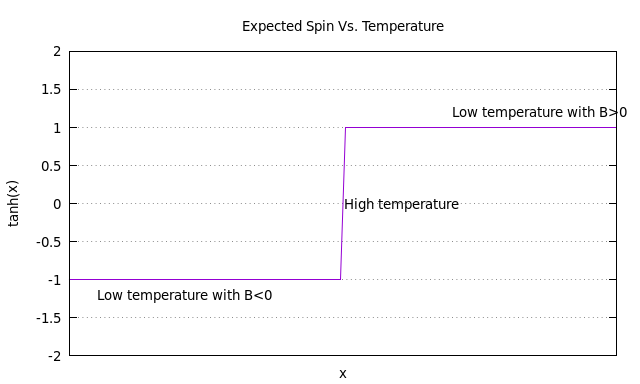
\includegraphics[width=\textwidth]{Figures/tanh.png}
\caption{Variation of average spin in a region with temperature ($\beta = 1/_T$)}
\end{figure}
From Fig. 1, it can be observed that at low temperatures ($\beta \to \infty$) all the spins are either up or down depending on the external magnetic field ($B$). However, at high temperatures ($\beta \to 0$) the spins are random due to which the average spin $\langle \sigma_{i}\rangle \to 0$. Summarising, the expected value of any spin in a region $\mathbb{L}$,	
	\[\langle\sigma_{i}\rangle =
	\begin{cases}
	\tanh(x), & \quad \text{for } \beta \to 0 \\
	\tanh(Nx), & \quad \text{for } \beta \to \infty
	\end{cases}	\]
\end{defn}
\begin{defn}[Average Magnetization] The extent of alignment in a region due to an external magnetic field ($B$) is given by average magnetization,
	$$M_{N}(\beta,B)=\frac{1}{N}\sum_{i\in \mathbb{L}}\langle\sigma_{i}\rangle$$
$M_{N}(\beta,B)$ is an odd function of $B$ due to the symmetry between up and down directions, as a consequence, $M_{N}(\beta,0) = 0$. 

\end{defn}

\begin{defn}[Spontaneous Magnetization] The alignment in a region due to an external magnetic field can be analysed using spontaneous magnetization,
$$M_{+}(\beta) = \lim \limits_{B \rightarrow 0^{+}}\limits \lim_{N\rightarrow\infty}M_{N}(\beta,B).$$
A few remarks about spontaneous magnetization,
\begin{enumerate}
	\item At low temperatures ($\beta \to \infty$) with $B \to 0^{+}$, the alignment of spins is $\sigma^{+} = (\sigma_{i} = 1,~\forall i)$ due to which $M_{+}(\infty) = 1$
	\item At high temperatures ($\beta \to 0$), the alignment of spins are random due to which $M_{+}(0) = 0$
	\item The critical temperature $T_{c} = 1/\beta_{c}$ is the one at which  a transition in the phase of the system occurs
	\item Spontaneous magnetization is always zero in the high temperature phase $\forall d$ (Paramagnetic Phase)
	\item In one-dimensional systems ($d=1$), a phase transition occurs at $T_{c} = 0 \implies M_{+}(\infty) = 0,~\forall \beta < \beta_{c}$
	\item For $d\geq 2$, the critical temperature is non-zero, and $M_{+}(\beta)>0$, $\forall \beta > \beta_{c}(d)$
	\end{enumerate}
\end{defn}

\subsection{The one-dimensional case}
\begin{figure}[hb]
\centering
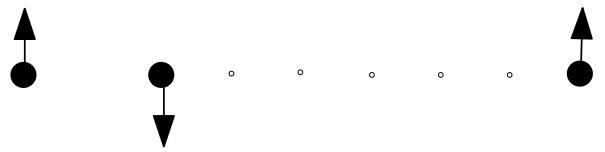
\includegraphics[width=\textwidth]{Figures/oned.png}
\caption{Illustration of an one-dimensional model with sites and their respective spins (arrows)}
\end{figure}
Consider a one-dimensional system ($d=1$) of $N$ spins, with energy ($E(\underline{\sigma})$)
$$E(\underline{\sigma})=-\sum_{i=1}^{N-1}\sigma_{i}\sigma_{i+1}-B\sum_{i=1}^{N}\sigma_{i}.$$
The partial partition function where the configurations of all spins $\sigma_{1},\cdots,\sigma_{p}$ have been summed over, at fixed $\sigma_{p+1}$:
\begin{equation}
z_{p}(\beta,B,\sigma_{p+1})=\sum_{\sigma_{1},\hdots,\sigma_{p}}\exp\bigg[\beta\sum_{i=1}^{p}\sigma_{i}\sigma_{i+1}+\beta B \sum_{i=1}^{p}\sigma_{i}\bigg].
\label{one}
\end{equation}
Expressing \eqref{one} recursively,
$$z_{p}(\beta,B,\sigma_{p+1})=\sum_{\sigma_{p}}\exp\bigg[\beta \sigma_{p}\sigma_{p+1}+\beta B \sigma_{p}\bigg]\sum_{\sigma_{1},\hdots,\sigma_{p-1}}\exp\bigg[\beta\sum_{i=1}^{p-1}\sigma_{i}\sigma_{i+1}+\beta B \sum_{i=1}^{p-1}\sigma_{i}\bigg],$$
$$z_{p}(\beta,B,\sigma_{p+1})= \sum_{\sigma_{p}=\pm 1} T(\sigma_{p+1},\sigma_{p})z_{p}(\beta,B,\sigma_{p}),$$ 
where $T(\sigma_{p+1},\sigma_{p}):= \exp[\beta \sigma_{p+1} \sigma_{p}+\beta B \sigma_{p}]$ is a $2 \times 2$ transfer matrix:
$$T = 
\begin{bmatrix}
	e^{\beta+\beta B} & e^{-\beta-\beta B} \\
	e^{-\beta+\beta B} & e^{\beta-\beta B} 
	\end{bmatrix}.$$
The partition function of the system with $N$ spins can be written using \eqref{one} as

$$Z_{N}(\beta,B)=\sum_{\sigma_{N}}z_{N-1}(\beta,B,\sigma_{N})\exp(\beta B\sigma_{N}).$$
Introducing the scalar product between two vectors as $(a,b) = a_{1}b_{1}+a_{2}b_{2}$, the partition function can now be expressed in matrix form as,
\begin{equation}
Z_{N}(\beta,B) = (\psi_{L},T^{N-1}\psi_{R}),
\label{seven}
\end{equation}
where, $\psi_{L} = \begin{bmatrix}  \exp(\beta B)\\ \exp(-\beta B)\end{bmatrix}$ and $\psi_{R} = \begin{bmatrix} 1\\ 1\end{bmatrix}$. The eigenvalues of the transfer matrix $T$ are,
\begin{equation}
\lambda_{1,2} = e^{\beta}\cosh(\beta B)\pm \sqrt{e^{2\beta} \sinh^{2}(\beta B) + e^{-2\beta}}.
\label{eight}
 \end{equation}
Let $\psi_{1}$ and $\psi_{2}$ be the corresponding eigenvectors, then, 
 \begin{equation}
\psi_{R} = u_{1}\psi_{1}+u_{2}\psi_{2}.
\label{nine}
 \end{equation}
 Using \eqref{eight} and \eqref{nine} in \eqref{seven} we have,
 \begin{align}
Z_{N}(\beta,B) &= \left(\psi_{L}, 
\begin{bmatrix}
	\lambda_{1}^{N-1} & 0 \\
	0 & \lambda_{2}^{N-1} 
	\end{bmatrix}\begin{bmatrix}
	u_{1} & 0 \\
	0 & u_{2} 
	\end{bmatrix}\begin{bmatrix} \psi_{1}\\ \psi_{2}\end{bmatrix} \right),\nonumber\\
Z_{N}(\beta,B) &= \left(\psi_{L}, 
\begin{bmatrix}
	\lambda_{1}^{N-1}u_{1} & 0 \\
	0 & \lambda_{2}^{N-1}u_{2} 
	\end{bmatrix}\begin{bmatrix} \psi_{1}\\ \psi_{2}\end{bmatrix} \right),\nonumber\\
Z_{N}(\beta,B) &= u_{1}(\psi_{L},\psi_{1})\lambda_{1}^{N-1}+u_{2}(\psi_{L},\psi_{2})\lambda_{2}^{N-1}.
\label{ten}
\end{align}
\begin{defn}[Free Entropy Density] It is given by 
\begin{align}
\phi(\beta,B) &= \lim \limits_{N\rightarrow\infty}\frac{1}{N}\phi_{N}(\beta,B),\nonumber\\
\phi(\beta,B) &=\lim \limits_{N\rightarrow\infty}\frac{1}{N}\log Z_{N}(\beta,B)\nonumber
\end{align}
However, for finite $\beta$, in the large $N$ limit, the partition function is dominated by the largest eigenvalue $\lambda_{1}$, and therefore 
\begin{equation}
\phi(\beta,B) = \log \lambda_{1}.
\label{lvn}
\end{equation}
\end{defn}

\begin{defn}[Expected Spin] Using the transfer matrix we can compute the expected value of a spin;
\begin{align}
\langle \sigma_{i}\rangle &= \sum_{\sigma} P(\sigma_{i})\sigma_{i},\nonumber\\
&= \frac{\sigma_{i}\exp\left(\beta\sum_{j=1}^{N-1}\sigma_{j}\sigma_{j+1}+\beta B \sum_{j=1}^{N}\sigma_{j}\right)}{Z(\beta)},\nonumber\\
&= \sum_{\sigma_{1},\sigma_{2},\ldots,\sigma_{N}}z_{i-1}(\beta,B,i)\sigma_{i}\exp\left(\beta \sum_{j=i}^{N-1}\sigma_{j}\sigma_{j+1}+\beta B \sum_{j=i}^{N}\sigma_{j}\right),\nonumber\\
\langle \sigma_{i}\rangle &= \frac{1}{Z_{N}(\beta,B)}(\psi_{L},T^{i-1}\hat{\sigma}T^{N-i}\psi_{R}),
\label{twlv}
\end{align}
where, $\hat{\sigma} = \begin{bmatrix} 1 & 0 \\ 0 & -1\end{bmatrix}$.
\end{defn}

\begin{defn}[Average Magnetization] It can be computed by averaging over alignments in a region. 
We know that,
\begin{align}
M_{N}(\beta,B) &= \frac{1}{N}\sum_{i=1}^{N}\langle\sigma_{i}\rangle,\nonumber\\
\text{Simplifying \eqref{twlv} and using \eqref{ten}},\nonumber\\
M_{N}(\beta,B) &= \frac{1}{N} \sum_{i=1}^{N} \left(\frac{u_{1}(\psi_{L},\psi_{1})\lambda_{1}^{N-1}-u_{2}(\psi_{L},\psi_{2})\lambda_{2}^{N-1}}{u_{1}(\psi_{L},\psi_{1})\lambda_{1}^{N-1}+u_{2}(\psi_{L},\psi_{2})\lambda_{2}^{N-1}}\right),\nonumber
\end{align}
In the thermodynamic limit, 
\begin{equation}
\lim \limits_{N\rightarrow\infty}M_{N}(\beta,B) = \frac{\sinh (\beta B)}{\sqrt{\sinh^{2}(\beta B)+e^{-4\beta}}} = \frac{1}{\beta}\frac{\partial \phi}{\partial B}(\beta,B).
\end{equation}
This relation can be easily verified using \eqref{lvn},
\begin{align}
\frac{1}{\beta}\frac{\partial \phi}{\partial B}(\beta,B) &= \frac{1}{\beta \lambda_{1}}\left(\beta e^{\beta}\sinh(\beta B)+\frac{2\beta e^{\beta}\sinh(\beta B)\cosh(\beta B)}{\sqrt{\sinh^{2}(\beta B)+e^{-4\beta}}}\right),\nonumber\\
&= \frac{\beta \sinh(\beta B)}{\beta \lambda_{1}}\left(\frac{\lambda_{1}}{\sqrt{\sinh^{2}(\beta B)+e^{-4\beta}}}\right),\nonumber\\
\frac{1}{\beta}\frac{\partial \phi}{\partial B}(\beta,B) &=\frac{\sinh (\beta B)}{\sqrt{\sinh^{2}(\beta B)+e^{-4\beta}}}.\nonumber
\end{align}
For $\beta < \infty$, the average magnetization is an analytic function of $\beta$ and $B$. At any non-zero temperature, the spontaneous magnetization is zero,
$$M_{+}(\beta) = 0,~\forall \beta < \infty.$$

\begin{defn}[Susceptibility]
Intuitively, susceptibility is the tendency of a site in a region to have the same alignment as its neighbors. The susceptibility associated with average magnetization is given by,
\begin{equation}
\chi_{M}(\beta)=\frac{\partial M}{ \partial B}(\beta,0) = \beta e^{2\beta}.
\end{equation}
The system behaves like the spins were blocked into groups of $^\chi(\beta)/_\beta$ spins each. The spins in each group are restricted to a value, while spins in different groups are independent. For $B=0$ and $\delta N<i<j<(1-\delta)N$, one finds at large $N$, 

$$\langle \sigma_{i}\sigma_{j}\rangle = e^{-|i-j|/\xi(\beta)}+ \Theta (e^{-\alpha N}),$$
where, $\xi(B) = \frac{-1}{\log \tanh \beta}$ is the distance below which two spins are well correlated, and is called the correlation length of the model. This length increases with decrease in temperature, that is, spins become more correlated at lower temperatures. The relation between correlation length and susceptibility is given by,
\begin{equation}
\chi_{M}(\beta)=\beta \sum_{i=-\infty}^{\infty}e^{\frac{-|i|}{\xi(\beta)}}+\Theta(e^{-\alpha N}).
\end{equation}
This makes it evident that a large susceptibility must correspond to a large correlation length. 
	\end{defn}
\end{defn}
\subsection{The Curie-Weiss Model}

The exact solution of the one-dimensional model, lead Ising to think that there couldn’t be a phase transition in any dimension. This was debunked by a qualitative theory of ferromagnetism which was put forward by Pierre Curie. It assumed the existence of a phase transition at non-zero temperature $T_{c}$ (Curie point) and a non-vanishing spontaneous magnetization for $T<T_{c}$. The dilemma was eventually solved by Onsager solution of the two-dimensional model. 

Consider $N$ Ising spins $\sigma_{i}\in \{\pm 1\}$ and a configuration $\sigma = (\sigma_{1},\hdots,\sigma_{N})$. Unlike the Ising model, the spins are not a part of a $d-$dimensional lattice, instead, they all interact in pairs. The absence of any finite-dimensional geometrical structure makes the Curie-Weiss model one among the mean-field models. The energy function, in the presence of a magnetic field $B$, is given by:
$$E(\underline{\sigma}) = -\frac{1}{N}\sum_{(ij)}\sigma_{i}\sigma_{j}-B\sum_{i=1}^{N}\sigma_{i}.$$ 
It needs to be mentioned that the summation over $(ij)$ involves $O(N^{2})$ terms of order $O(1)$. Therefore, the energy function is scaled by $^1/_N$ to obtain a non-trivial free-energy density in the thermodynamic limit. The instantaneous magnetization which is a function of the configuration:
$$m(\underline{\sigma}) = \frac{1}{N}\sum_{i=1}^{N}\sigma_{i}.$$


\end{document}

